\section{User Guide}
\label{sec:user_guide}

This section describes how to configure, run, and monitor the \textsc{Debate2Rescue} simulation. It details system requirements, startup configuration, the graphical user interface (GUI), runtime controls, and debate log files.

% -----------------------------------------------------------------------------
\subsection{Getting Started}
\label{subsec:getting_started}
% -----------------------------------------------------------------------------

\subsubsection{Prerequisites}
The simulation requires:
\begin{itemize}
    \item \textbf{Java Development Kit (JDK):} Version 21 or higher.
    \item \textbf{Gradle:} The repository bundles the Gradle wrapper (\texttt{gradlew}), so a separate local Gradle installation is not required.
    \item \textbf{Operating System:} Linux, macOS, or Windows with graphical desktop support.
\end{itemize}

\subsubsection{Running the Simulation}
To launch the simulation with default settings, run from the project root:
\begin{verbatim}
./gradlew run
\end{verbatim}
or on Windows:
\begin{verbatim}
gradlew.bat run
\end{verbatim}

On startup, a configuration dialog opens before initializing the agents and grid environment.

% -----------------------------------------------------------------------------
\subsection{Initial Configuration}
\label{subsec:initial_config}
% -----------------------------------------------------------------------------

The startup dialog (\texttt{SimConfigDialog}, \Cref{fig:config_dialog}) allows configuring the grid dimensions and agent population.

\begin{figure}[htbp]
    \centering
    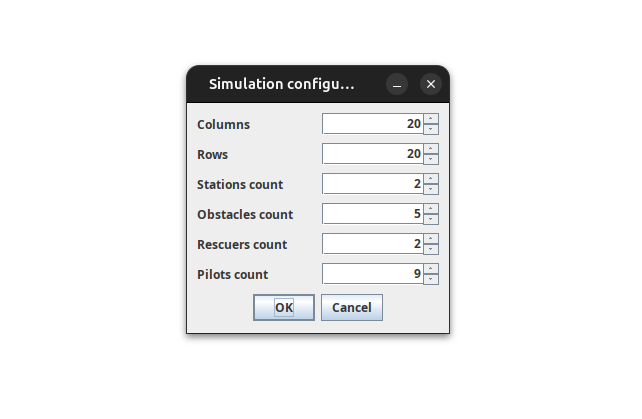
\includegraphics[width=0.45\textwidth]{figures/sim_config_dialog.png}
    \caption{Simulation configuration dialog.}
    \label{fig:config_dialog}
\end{figure}

The configurable parameters and ranges are summarized in \Cref{tab:initial_config_params}.

\begin{table}[htbp]
\centering
\small
\begin{tabular}{|l|c|c|p{5.5cm}|}
\hline  
\textbf{Parameter} & \textbf{Default} & \textbf{Range} & \textbf{Description} \\
\hline
\textbf{Columns} & 20 & 10 -- 50 & Grid width. \\
\textbf{Rows} & 20 & 10 -- 50 & Grid height. \\
\textbf{Stations} & 2 & 1 -- MaxStations & Number of base stations. \\
\textbf{Obstacles} & 5 & 0 -- MaxObstacles & Number of obstacle cells. \\
\textbf{Rescuers} & 2 & 1 -- MaxRescuers & Number of rescuer agents. \\
\textbf{Pilots} & 9 & MinPilots -- MaxPilots & Number of resource pilots. \\
\hline
\end{tabular}
\caption{Initial configuration parameters.}
\label{tab:initial_config_params}
\end{table}

\subsubsection{Validation Rules and Default Values}
The dialog enforces several constraints based on the average grid dimension $M$ based on the grid width and height:
\begin{itemize}
    \item \textbf{Base stations:} Defaults to $\mathrm{round}(0.10 \times M)$ with an upper limit of $\mathrm{round}(0.50 \times M)$.
    \item \textbf{Obstacles:} Defaults to $\mathrm{round}(0.25 \times M)$ with an upper limit of $\mathrm{round}(1.00 \times M)$.
    \item \textbf{Rescuers:} At least one rescuer per station, up to a maximum of four per station ($\mathrm{stations} \le \mathrm{rescuers} \le 4 \times \mathrm{stations}$). The default assigns one rescuer per station.
    \item \textbf{Pilots:} Bounded between $\max(\mathrm{stations}, 9)$ and $4 \times \mathrm{stations}$, ensuring that every station has at least one pilot and that each of the nine resource types (helicopter, fire truck, ambulance, police car, excavator, police helicopter, army, bomb squad, hazmat team) has an assigned pilot.
\end{itemize}

% -----------------------------------------------------------------------------
\subsection{Graphical User Interface}
\label{subsec:gui_overview}
% -----------------------------------------------------------------------------

After configuration, the main application window is displayed (\Cref{fig:main_gui}). It is divided into two sections:
\begin{enumerate}
    \item \textbf{Grid Canvas (Left):} A 2D grid rendering the environment, stationary structures, and mobile agents.
    \item \textbf{Side Panel (Right):} Hosts runtime controls, the visual legend, and two real-time logging panes.
\end{enumerate}

\begin{figure}[htbp]
    \centering
    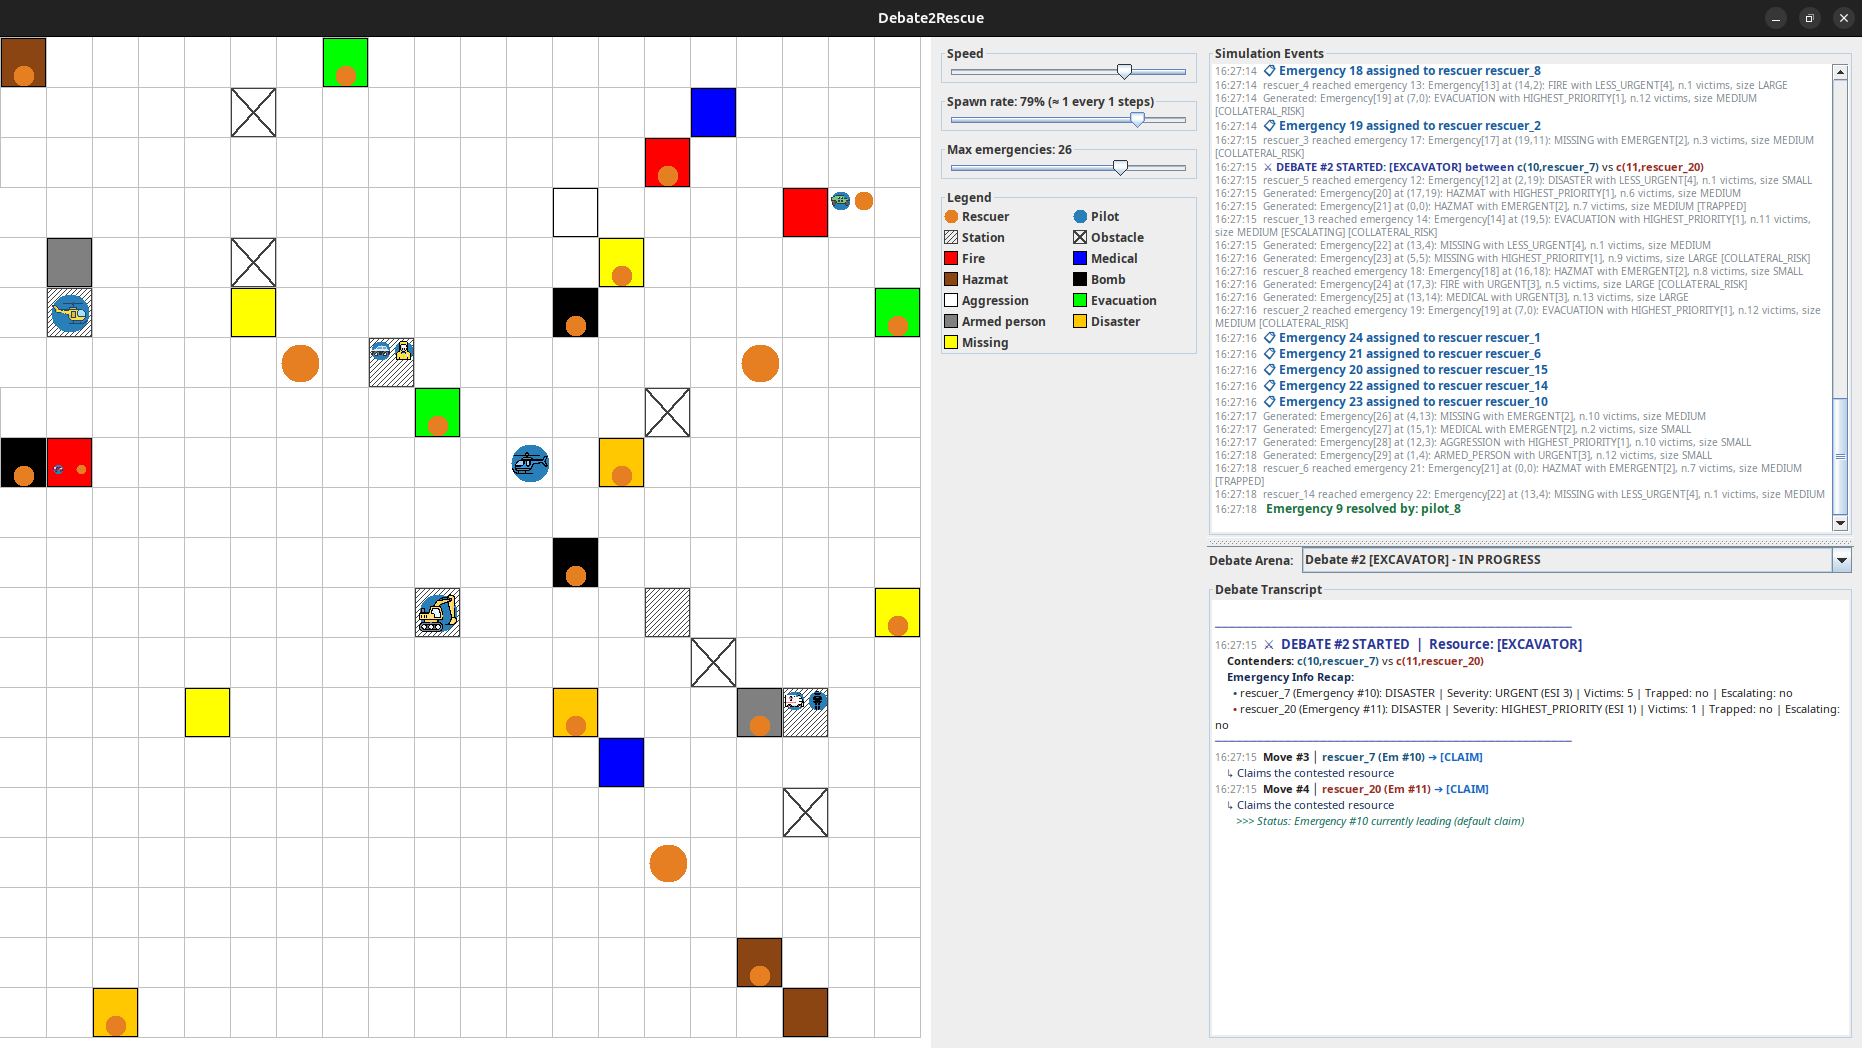
\includegraphics[width=0.95\textwidth]{figures/main_gui.png}
    \caption{The main graphical user interface of \textsc{Debate2Rescue}.}
    \label{fig:main_gui}
\end{figure}

\subsubsection{Grid Elements}
The canvas displays entities using distinct shapes and colors:
\begin{itemize}
    \item \textbf{Base Stations:} Gray cells with diagonal stripes, representing bases where responders wait between assignments.
    \item \textbf{Obstacles:} White cells with a dark cross, representing impassable cells.
    \item \textbf{Emergencies:} Colored squares, color-coded by emergency category.
    \item \textbf{Responders:} Circles representing rescuer and pilot agents, color-coded by role.
\end{itemize}
A visual legend at the bottom-left of the side panel maps each icon and color to its corresponding entity or emergency type.

\subsubsection{Cell Tooltips}
Hovering the cursor over any station or emergency cell displays a tooltip with details such as emergency status, severity level (and ESI score), victim count, station presence, and any responders currently on the cell.

% -----------------------------------------------------------------------------
\subsection{Runtime Simulation Controls}
\label{subsec:runtime_config}
% -----------------------------------------------------------------------------

Three sliders at the top of the side panel allow adjusting simulation parameters dynamically during execution (\Cref{fig:sliders}):
\begin{itemize}
    \item \textbf{Speed:} Controls step execution delay; moving the slider to the right increases simulation speed.
    \item \textbf{Spawn rate:} Controls the per-step probability of spawning a new emergency ($0\%$ to $100\%$). Setting it to $0\%$ disables new emergency generation.
    \item \textbf{Max emergencies:} Sets the upper limit on concurrent active emergencies in the grid.
\end{itemize}

\begin{figure}[htbp]
    \centering
    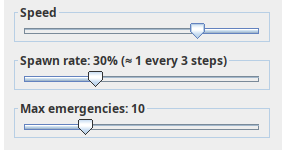
\includegraphics[width=0.4\textwidth]{figures/sliders.png}
    \caption{Runtime adjustment sliders in the side panel.}
    \label{fig:sliders}
\end{figure}

% -----------------------------------------------------------------------------
\subsection{Real-Time Logging}
\label{subsec:gui_logging}
% -----------------------------------------------------------------------------

The side panel features two vertically split logging panes: the upper pane logs general simulation events, while the lower pane streams debate transcripts.

\begin{figure}[htbp]
    \centering
    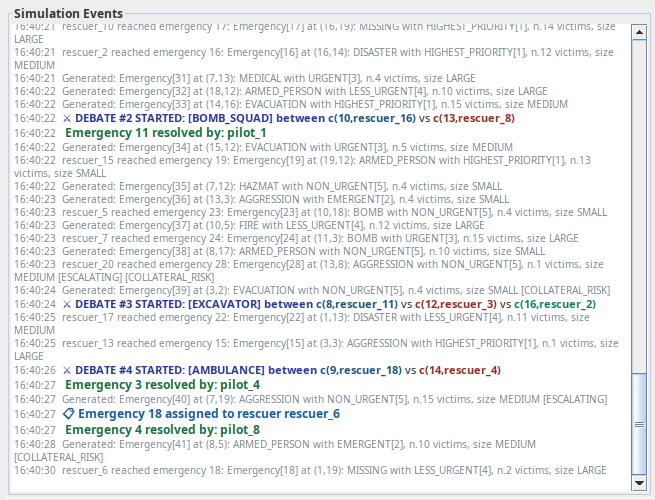
\includegraphics[width=0.55\textwidth]{figures/simulation_events.png}
    \caption{Simulation events log (top pane).}
    \label{fig:simulation_events}
\end{figure}

\subsubsection{Simulation Events Pane}
The upper pane logs environment and multi-agent lifecycle events in real time (\Cref{fig:simulation_events}):
\begin{itemize}
    \item \textbf{Routine grid events:} Actions already visible on the canvas (agent movement, emergency spawn, agent registration) are shown in muted gray to reduce clutter.
    \item \textbf{Task coordination events:} Highlighted with icons and colors:
    \begin{itemize}
        \item \texttt{[Assign]} (blue): Emergency assignment sent to a rescuer.
        \item \texttt{[Resolve]} (green): Emergency successfully resolved.
        \item \texttt{[Message]} (dark text): Direct inter-agent communication.
    \end{itemize}
    \item \textbf{Debate summaries:} One-line notices marking the start and conclusion of each resource debate, indicating the debate ID, contested resource, and winner.
\end{itemize}

\subsubsection{Debate Arena Pane}
The lower pane records the argumentation dialogue whenever two or more rescuers compete for the same specialized resource via Arg2P (\Cref{fig:debate_arena}).

\begin{figure}[htbp]
    \centering
    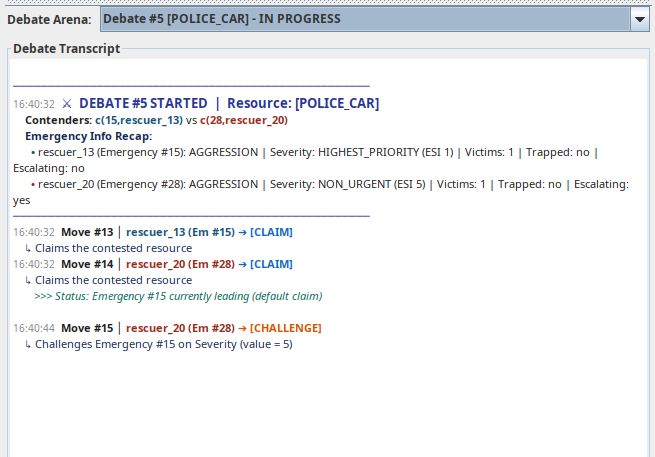
\includegraphics[width=0.55\textwidth]{figures/debate_arena.png}
    \caption{Debate arena transcript (bottom pane).}
    \label{fig:debate_arena}
\end{figure}

The Debate Arena contains:
\begin{itemize}
    \item \textbf{Session selector:} A dropdown menu to switch between active and concluded debates (most recent first).
    \item \textbf{Header:} Summarizes the contested resource and contender emergency profiles (severity, victim count, trapped victims, escalation status).
    \item \textbf{Dialogue turns:} Color-coded by performative:
    \begin{itemize}
        \item \textbf{\textcolor{blue}{CLAIM:}} Resource request by an agent.
        \item \textbf{\textcolor{orange}{CHALLENGE:}} Attack on an opponent's priority based on criteria such as severity or victim count.
        \item \textbf{\textcolor{violet}{ANSWER:}} Response or counter-argument defending an emergency.
        \item \textbf{\textcolor{red}{CONCEDE:}} Concession withdrawing a claim when an opponent's argument dominates.
    \end{itemize}
    \item \textbf{Turn status:} Updates after each move to display the current leader and the applied ranking rule.
    \item \textbf{Debate summary:} Concluding banner showing the winning emergency, the assigned rescuer, the final justification, and any conceded contenders.
\end{itemize}

% -----------------------------------------------------------------------------
\subsection{Persistent File Logs}
\label{subsec:persistent_logs}
% -----------------------------------------------------------------------------

Each debate session is saved to disk for inspection and offline analysis.

\subsubsection{Directory Structure and File Naming}
On each run, a timestamped directory is created under \texttt{logs/}:
\[
\texttt{logs/yyyy-MM-dd\_HH-mm-ss/}
\]
Each debate produces an individual log file named:
\[
\texttt{debate<ID>\_<resource\_type>.log}
\]
For example, \texttt{debate1\_fire\_truck.log}.

\subsubsection{Log File Structure}
Each log file contains three parts:
\begin{enumerate}
    \item \textbf{Header:} Start timestamp, contested resource, and contender profiles (emergency ID, severity, victim count, trapped victims, and escalation status).
    \item \textbf{Moves log:} Timestamped record of each argumentative move and the intermediate leading state with its ranking rule.
    \item \textbf{Footer:} Final decision, winner, conceded contenders, deciding justification, and total move count.
\end{enumerate}

A sample debate log is shown in \Cref{fig:sample_debate_log}.

\begin{figure}[htbp]
\centering
\begin{minipage}{0.95\textwidth}
\footnotesize
\begin{verbatim}
=================================================================
DEBATE #1 STARTED: Resource Type [fire_truck]
Timestamp: 2026-10-28 14:35:45
Contenders: c(7,rescuer_15), c(10,rescuer_13)

Contender Emergency Infos:
  * rescuer_15 (Emergency #7): FIRE | Severity: LESS_URGENT (ESI 4)
    | Victims: 12 | Trapped: no | Escalating: no
  * rescuer_13 (Emergency #10): FIRE | Severity: LESS_URGENT (ESI 4)
    | Victims: 2  | Trapped: no | Escalating: no
=================================================================

--- DEBATE MOVES & TURNS ---
[2026-10-28 14:35:45] Move #1: rescuer_15 (Emergency 7)  -> CLAIM: claim
[2026-10-28 14:35:45] Move #2: rescuer_13 (Emergency 10) -> CLAIM: claim
       >>> Status: Leading Emergency = 7 | Reason: []

[2026-10-28 14:35:54] Move #5: rescuer_13 (Emergency 10) -> CHALLENGE:
       challenge(7,severity,4)
       >>> Status: Leading Emergency = 10 | Reason: [rank(severity,10,7)]

[2026-10-28 14:36:07] Move #12: rescuer_15 (Emergency 7) -> ANSWER:
       answer(5,severity,4)
       >>> Status: Leading Emergency = 7 | Reason: []

[2026-10-28 14:36:33] Move #15: rescuer_13 (Emergency 10) -> CHALLENGE:
       challenge(7,size,2)
       >>> Status: Leading Emergency = 10 | Reason: [rank(size,10,7)]

[2026-10-28 14:37:30] Move #22: rescuer_15 (Emergency 7) -> ANSWER:
       answer(15,size,3)
       >>> Status: Leading Emergency = 7 | Reason: [rank(size,7,10)]

[2026-10-28 14:38:33] Move #30: rescuer_13 (Emergency 10) -> CONCEDE:
       "withdrew claim"
       >>> Status: Leading Emergency = 7 | Reason: []

=================================================================
DEBATE #1 CONCLUDED: Resource Type [fire_truck]
Timestamp: 2026-10-28 14:38:33
FINAL DECISION: Winner is Emergency 7
DENIED CONTENDERS: c(10,rescuer_13) [conceded]
JUSTIFICATION: All opponent(s) conceded (deciding argument: size)
TOTAL MOVES: 30
=================================================================
\end{verbatim}
\end{minipage}
\caption{Excerpt of a persistent debate log file (\texttt{debate1\_fire\_truck.log}).}
\label{fig:sample_debate_log}
\end{figure}
